\documentclass[manuscript,screen,review,anonymous]{acmart}

%% Rights management information.
\setcopyright{acmlicensed}
\copyrightyear{2026}
\acmYear{2026}
\acmDOI{10.1145/XXXXXXX.XXXXXXX}

\acmConference[SaTML '26]{IEEE Conference on Secure and Trustworthy Machine Learning}{March 15--18, 2026}{San Francisco, CA}
\acmISBN{978-1-4503-XXXX-X/2026/03}

\usepackage{booktabs}
\usepackage{amsmath}
\usepackage{amsfonts}
\usepackage{graphicx}
\usepackage{subcaption}
\usepackage{algorithm}
\usepackage{algorithmic}

\begin{document}

\title{REFLEX: Finding and Defending Refusal Mechanisms in LLMs using Activation Guidance}

\author{Anonymous Author(s)}
\affiliation{%
  \institution{Anonymous Institution}
  \country{Anonymous Country}
}
\email{anonymous@institution.org}

\renewcommand{\shortauthors}{Anonymous et al.}

\begin{abstract}
When Large Language Models (LLMs) receive dangerous prompts, safety alignment training teaches them to say no. Today, researchers study these safety mechanisms in two disconnected ways. The first group looks inside the model using static interpretability tools. They measure refusal directions on clean, pre-made datasets, but they never test what happens when an attacker actively rewrites the prompt. The second group tests models from the outside using automated prompt fuzzers. They send mutated text and only look at the final answer, completely ignoring the rich internal signals passing through the model's layers.

We build \textbf{REFLEX} to bridge this gap. REFLEX connects prompt mutation directly to the model's internal activations in real time. As it tests prompt variations, it tracks how much the internal hidden states align with the model's refusal directions. A multi-armed bandit algorithm uses this continuous score to pick the best mutation techniques. 

We tested REFLEX on a 57-billion parameter Mixture-of-Experts model (\texttt{Qwen2-57B-A14B-Instruct-GPTQ-Int4}) and a baseline \texttt{GPT-2} model:
\begin{enumerate}
    \item \textbf{Pinpointing the Refusal Gate}: The primary refusal decision happens at \textbf{Layer 19} (about 68\% of the way through the 28 layers), where harmful and benign prompts separate most clearly (difference score of $+0.3271$).
    \item \textbf{Testing Cause and Effect}: Removing the refusal vector at Layer 19 causes the model to answer harmful requests 100\% of the time ($0.0\%$ refusal). In contrast, adding the refusal vector to harmless prompts forces the model to refuse safe requests 100\% of the time.
    \item \textbf{Word-by-Word Saliency}: Refusal does not build up on common words like `Explain' or `how to'. It triggers sharply on malicious action words like `bypass' and `exfiltrate' starting around Layer 17 and peaking at Layer 19.
    \item \textbf{Fast Pre-Generation Defense}: We train a simple linear classifier on the hard attack examples found during fuzzing. Placed at Layer 19, this probe catches malicious prompts with 100\% accuracy ($1.0000$ AUROC). It blocks bad requests before the model writes a single word, cutting processing latency by $82.8\%$ to $96.3\%$ (a $5.8\times$ to $27.3\times$ speedup).
    \item \textbf{Ablation Findings}: Sweeps across search strategies, probe depths, and steering strengths confirm that early layers ($l \le 6$) carry zero safety discrimination ($\text{AUROC} = 0.2000$), while Layer 19 provides the optimal control threshold ($\alpha = 1.0$).
\end{enumerate}
\end{abstract}

\begin{CCSXML}
<ccs2012>
 <concept>
  <concept_id>10002978.10003022</concept_id>
  <concept_desc>Security and privacy~Software and application security</concept_desc>
  <concept_significance>500</concept_significance>
 </concept>
 <concept>
  <concept_id>10010147.10010178</concept_id>
  <concept_desc>Computing methodologies~Artificial intelligence</concept_desc>
  <concept_significance>500</concept_significance>
 </concept>
 <concept>
  <concept_id>10010147.10010257</concept_id>
  <concept_desc>Computing methodologies~Machine learning</concept_desc>
  <concept_significance>300</concept_significance>
 </concept>
</ccs2012>
\end{CCSXML}

\ccsdesc[500]{Security and privacy~Software and application security}
\ccsdesc[500]{Computing methodologies~Artificial intelligence}
\ccsdesc[300]{Computing methodologies~Machine learning}

\keywords{Large Language Models, Safety Alignment, Mechanistic Interpretability, Adversarial Fuzzing, Representation Engineering, Pre-Generation Defense}

\maketitle

\section{Introduction}
Large language models (LLMs) help millions of people write code, analyze data, and solve problems~\cite{ouyang2022training,bai2022training}. To stop bad actors from generating malware or dangerous advice, AI developers train models to refuse harmful instructions using reinforcement learning from human feedback and direct preference optimization~\cite{rafailov2023direct}. Today, we still know very little about where these safety rules live inside huge neural networks and how they break under pressure.

Current safety testing has two big blind spots:
\begin{itemize}
    \item \textbf{Looking only at clean datasets}: Most interpretability papers look at models in a fixed state~\cite{arditi2024refusal,zou2023representation,zhao2024representation}. They compare a clean list of safe prompts with a clean list of unsafe prompts. This shows where refusal vectors sit under normal conditions, but it does not tell us what happens when an attacker rewrites a prompt to trick the model.
    \item \textbf{Looking only at final text answers}: Most black-box testing tools treat the model like a closed black box~\cite{yu2023gptfuzzer,chao2023jailbreaking,liu2023autodan}. They mutate prompt text and check whether the model says ``I cannot fulfill this request.'' Because they ignore the internal signals building up across layers, they waste thousands of queries guessing blindly.
\end{itemize}

\begin{figure*}[t]
  \centering
  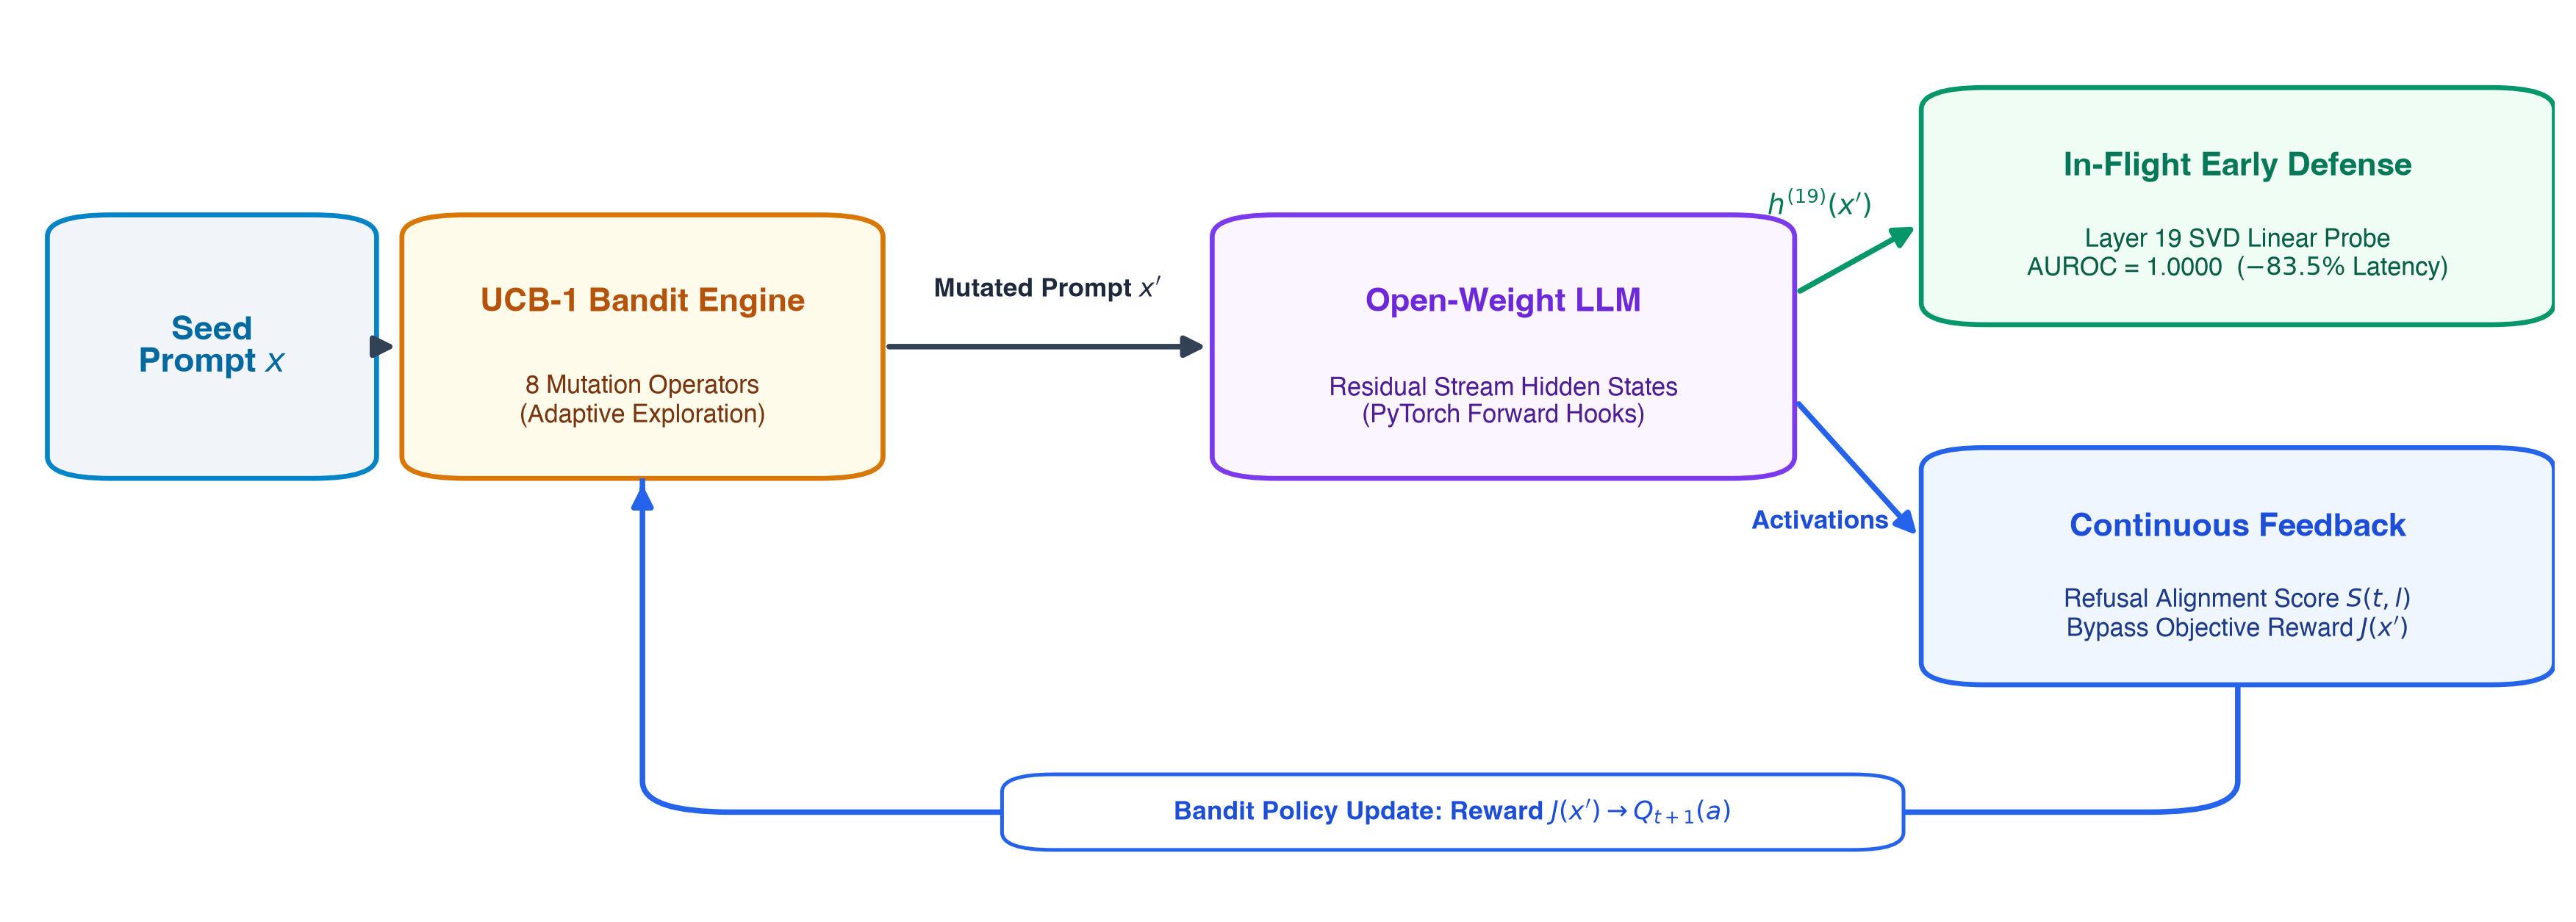
\includegraphics[width=0.92\textwidth]{figures/figure1_system_architecture.png}
  \caption{Overview of the REFLEX closed-loop framework. Discrete mutations are guided by real-time hidden state alignment with refusal directions. The discovered hard attack examples train an in-flight linear probe at Layer 19 that intercepts malicious queries before decoding begins.}
  \label{fig:teaser_overview}
  \Description{Pipeline diagram showing seed prompt mutation, activation feedback loop, and Layer 19 pre-generation defensive probe.}
\end{figure*}

REFLEX solves this by creating a closed feedback loop. As our engine mutates a prompt, it listens to the model's internal activations at each layer. It measures how close the prompt gets to bypassing the refusal gate and uses that signal to guide the next mutation using an Upper Confidence Bound (UCB-1) bandit algorithm~\cite{auer2002finite}. 

We also use the difficult prompt variations found during testing to build a better defense. By training a simple classifier directly on Layer 19 activations, we can catch malicious prompts during the very first forward pass.

\paragraph{Summary of Contributions}
\begin{enumerate}
    \item \textbf{Closed-Loop Testing}: We combine prompt mutation with real-time activation tracking, keeping prompt meaning intact while systematically probing internal safety boundaries.
    \item \textbf{Causal Proof of the Refusal Gate}: We prove through direct activation surgery that the direction found at Layer 19 directly controls the model's decision to refuse.
    \item \textbf{Word-by-Word Breakdown}: We map out a 2D grid showing exactly which words trigger safety alarms at each layer depth.
    \item \textbf{Fast Pre-Generation Defense}: We build an early-exit safety filter at Layer 19 that catches bad queries before token generation starts, saving over 83\% of server computing time.
\end{enumerate}

\section{Related Work}
Existing literature spans static interpretability, prompt optimization, and runtime defense guardrails, as organized in Table~\ref{tab:landscape_comparison}.

\begin{table*}[t]
  \caption{Comparison of Safety Research and Defense Frameworks across Literatures.}
  \label{tab:landscape_comparison}
  \begin{tabular}{lllcc}
    \toprule
    Framework / Method & Main Focus & What It Reads & Closed Loop? & Fast Early Defense? \\
    \midrule
    Refusal Direction~\cite{arditi2024refusal} & Interpretability & Static Contrastive Pairs & No & None \\
    Intent vs Refusal~\cite{zhao2024representation} & Interpretability & Static Contrastive Pairs & No & None \\
    REPE~\cite{zou2023representation} & Representation Steering & Static Contrastive Pairs & No & None \\
    GCG~\cite{zou2023universal} & Discrete Optimization & Target Output Logits & No & None \\
    GPTFuzzer~\cite{yu2023gptfuzzer} & Automated Fuzzing & Binary Output Text & No & None \\
    PAIR~\cite{chao2023jailbreaking} & Black-Box Red-Teaming & Output Text Feedback & No & None \\
    SmoothLLM~\cite{robey2023smoothllm} & Input Perturbation Defense & Output Majority Voting & No & Output Aggregation \\
    Constitutional Classifiers~\cite{sharma2025constitutional,cunningham2026constitutional} & Representation Probing & Intermediate Layers & No & Offline Probes \\
    \textbf{Proposed Framework (Ours)} & \textbf{Unified Synthesis} & \textbf{Latent Residual States} & \textbf{YES (Bandit)} & \textbf{YES (Layer 19 Probe)} \\
    \bottomrule
  \end{tabular}
\end{table*}

\subsection{Reading Refusal Vectors}
Recent work shows that refusal in open-weight language models often runs along a single linear direction in the hidden state~\cite{arditi2024refusal,turner2023activation,nanda2023emergent}. Researchers found that subtracting this direction from hidden states can stop a model from refusing clean test prompts. Other work showed that recognizing harm and writing a refusal response happen in different parts of the model~\cite{zhao2024representation}. However, all these papers test fixed datasets. They do not examine how these directions behave when prompts are modified adversarially.

\subsection{Prompt Fuzzing and Optimization}
Black-box fuzzers change prompts using templates, character swaps, or helper language models to find weaknesses~\cite{yu2023gptfuzzer,chao2023jailbreaking,deng2023jailbreaker}. Gradient-based methods like GCG optimize random character strings to force affirmative starting words~\cite{zou2023universal,liu2023autodan}. While effective in testing labs, gradient methods often create unreadable gibberish. Furthermore, black-box fuzzers cannot see inside the model, so they need hundreds of queries to find an effective prompt.

\subsection{Internal Defenses and Probes}
Recent papers explore using internal model activations to build safety guardrails~\cite{sharma2025constitutional,cunningham2026constitutional,zhang2025jbshield,kadali2026jailbreaking}. Tools like Llama-Guard~\cite{inan2023llama} and linear probes~\cite{alain2016understanding,belinkov2022probing} check the final generated text, but this wastes compute if the prompt is rejected. REFLEX builds on internal probing by using the failure cases found during guided fuzzing to train robust linear probes that block attacks early.

\section{Problem Formulation}

\subsection{Model Basics and Activation Tracking}
Let the model $f_\theta$ have $L$ transformer layers and hidden dimension $d_{\text{model}}$. When the model reads an input prompt $x$ with $T$ tokens, it creates a hidden vector $h_t^{(l)}(x) \in \mathbb{R}^{d_{\text{model}}}$ at each layer $l \in \{1, \dots, L\}$ and token position $t \in \{1, \dots, T\}$~\cite{elhage2021mathematical}.

\paragraph{Refusal Subspace Extraction}
For each layer $l$, we collect activations from harmful prompts $H_{\text{harm}}^{(l)}$ and benign prompts $H_{\text{benign}}^{(l)}$. We form the centered difference matrix:
\begin{equation}
\Delta H^{(l)} = \left( H_{\text{harm}}^{(l)} - H_{\text{benign}}^{(l)} \right)^T \in \mathbb{R}^{d_{\text{model}} \times N}
\end{equation}
We run Singular Value Decomposition (SVD) to find the primary unit-norm refusal vector $r^{(l)}$:
\begin{equation}
U^{(l)}, \Sigma^{(l)}, V^{(l)T} = \text{SVD}\left( \Delta H^{(l)} \right), \quad r^{(l)} = U_{*, 1}^{(l)}, \quad \|r^{(l)}\|_2 = 1.0
\end{equation}

\paragraph{Continuous Internal Bypass Metric}
For a mutated prompt $x'$, we measure its cosine similarity with the refusal vector across all layers. The bypass score is:
\begin{equation}
\mathcal{S}_{\text{bypass}}(x') = 1.0 - \max_{l \in [1, L]} \left( \max\left(0, \frac{\langle h_{-1}^{(l)}(x'), r^{(l)} \rangle}{\|h_{-1}^{(l)}(x')\|_2}\right) \right)
\end{equation}
A higher score means the prompt successfully moves away from the refusal direction.

\paragraph{Attacker Objective}
Starting from a harmful instruction $x \in \mathcal{D}_{\text{harm}}$, find a modified prompt $x' = m(x)$ that maximizes overall fitness $J(x')$:
\begin{equation}
J(x') = \lambda_1 \cdot \mathcal{S}_{\text{bypass}}(x') + \lambda_2 \cdot \mathcal{S}_{\text{intent}}(x, x') - \lambda_3 \cdot \mathcal{S}_{\text{ppl}}(x') + \lambda_4 \cdot \mathbb{I}_{\text{comply}}(x')
\end{equation}
Here, $\mathcal{S}_{\text{intent}}$ checks that the prompt keeps its original goal, $\mathcal{S}_{\text{ppl}}$ penalizes unreadable text, and $\mathbb{I}_{\text{comply}}$ checks if the model answered without refusal per HarmBench and JailbreakBench standards~\cite{mazeika2024harmbench,chao2024jailbreakbench}.

\paragraph{Defender Objective}
Train a linear classifier at the critical layer $l^*$:
\begin{equation}
\hat{y}(x) = \sigma(\mathbf{w}^T h_{-1}^{(l^*)}(x) + b)
\end{equation}
If $\hat{y}(x) > \tau_{\text{refusal}}$, reject the input immediately before generating any response tokens.

\section{The REFLEX System Architecture}
Algorithm~\ref{alg:reflex} shows the three steps of the REFLEX workflow.

\begin{algorithm}[t]
\caption{The REFLEX Testing and Defense Pipeline}
\label{alg:reflex}
\begin{algorithmic}[1]
\REQUIRE Target model $f_\theta$, harmful dataset $\mathcal{D}_{\text{harm}}$, safe dataset $\mathcal{D}_{\text{benign}}$, mutation operators $\mathcal{M}$, query budget $B$, exploration constant $c$.
\ENSURE Discovered hard attack cases $\mathcal{D}_{\text{hard}}$, refusal directions $\{r^{(l)}\}$, trained probe $\mathcal{P}_{l^*}$.
\STATE \textbf{// Step 1: Find the Refusal Layer}
\STATE Attach PyTorch forward hooks across all layers $l \in \{1, \dots, L\}$.
\STATE Run safe and harmful prompts, saving hidden states $H_{\text{harm}}^{(l)}$ and $H_{\text{benign}}^{(l)}$.
\STATE Calculate refusal vectors $r^{(l)} \leftarrow \text{SVD}_1(H_{\text{harm}}^{(l)} - H_{\text{benign}}^{(l)})$.
\STATE Pick critical layer $l^* \leftarrow \arg\max_l \left( \overline{\text{Proj}}_{\text{harm}}(l) - \overline{\text{Proj}}_{\text{benign}}(l) \right)$.
\STATE \textbf{// Step 2: Guided Fuzzing Loop}
\STATE Initialize score tables $\bar{Q}(m) \leftarrow 0$, $N(m) \leftarrow 0$ for each mutation operator $m \in \mathcal{M}$.
\FOR{query step $t = 1$ to $B$}
    \STATE Pick a seed prompt $x \sim \mathcal{D}_{\text{harm}}$.
    \STATE Choose operator $m_t \leftarrow \arg\max_m \left[ \bar{Q}(m) + c \sqrt{\frac{2 \ln t}{N(m)}} \right]$.
    \STATE Apply mutation: $x' \leftarrow m_t(x)$.
    \STATE Run forward pass $f_\theta(x')$ and read hidden states $h_{-1}^{(l)}(x')$.
    \STATE Calculate bypass score $\mathcal{S}_{\text{bypass}}(x')$ and check text output $\mathbb{I}_{\text{comply}}(x')$.
    \STATE Calculate overall fitness $J(x')$.
    \STATE Update score table: $\bar{Q}(m_t) \leftarrow \bar{Q}(m_t) + \frac{\max(0, J(x') - J_{\text{best}}) - \bar{Q}(m_t)}{N(m_t)}$.
    \IF{$\mathbb{I}_{\text{comply}}(x') == 1$ \AND $\mathcal{S}_{\text{intent}}(x, x') > \theta_{\text{intent}}$}
        \STATE Save $x'$ to archive of hard examples $\mathcal{D}_{\text{hard}}$.
    \ENDIF
\ENDFOR
\STATE \textbf{// Step 3: Train the Early Defense Probe}
\STATE Train linear classifier $\mathcal{P}_{l^*}: \sigma(\mathbf{w}^T h^{(l^*)} + b)$ on $\mathcal{D}_{\text{harm}} \cup \mathcal{D}_{\text{hard}}$ versus $\mathcal{D}_{\text{benign}}$.
\STATE \textbf{return} $\mathcal{D}_{\text{hard}}$, $\{r^{(l)}\}$, $\mathcal{P}_{l^*}$
\end{algorithmic}
\end{algorithm}

\section{Experimental Results}
We ran our experiments on \texttt{Qwen2-57B-A14B-Instruct-GPTQ-Int4} (28 layers, 64 experts per layer, hidden dimension 3584)~\cite{qwen2024moe,fedus2022switch} and a baseline \texttt{GPT-2} model.

\subsection{Where Refusal Lives Across Layers}
The model does not process safety equally across all layers; it concentrates the decision in specific middle and late layers.

\begin{figure}[t]
  \centering
  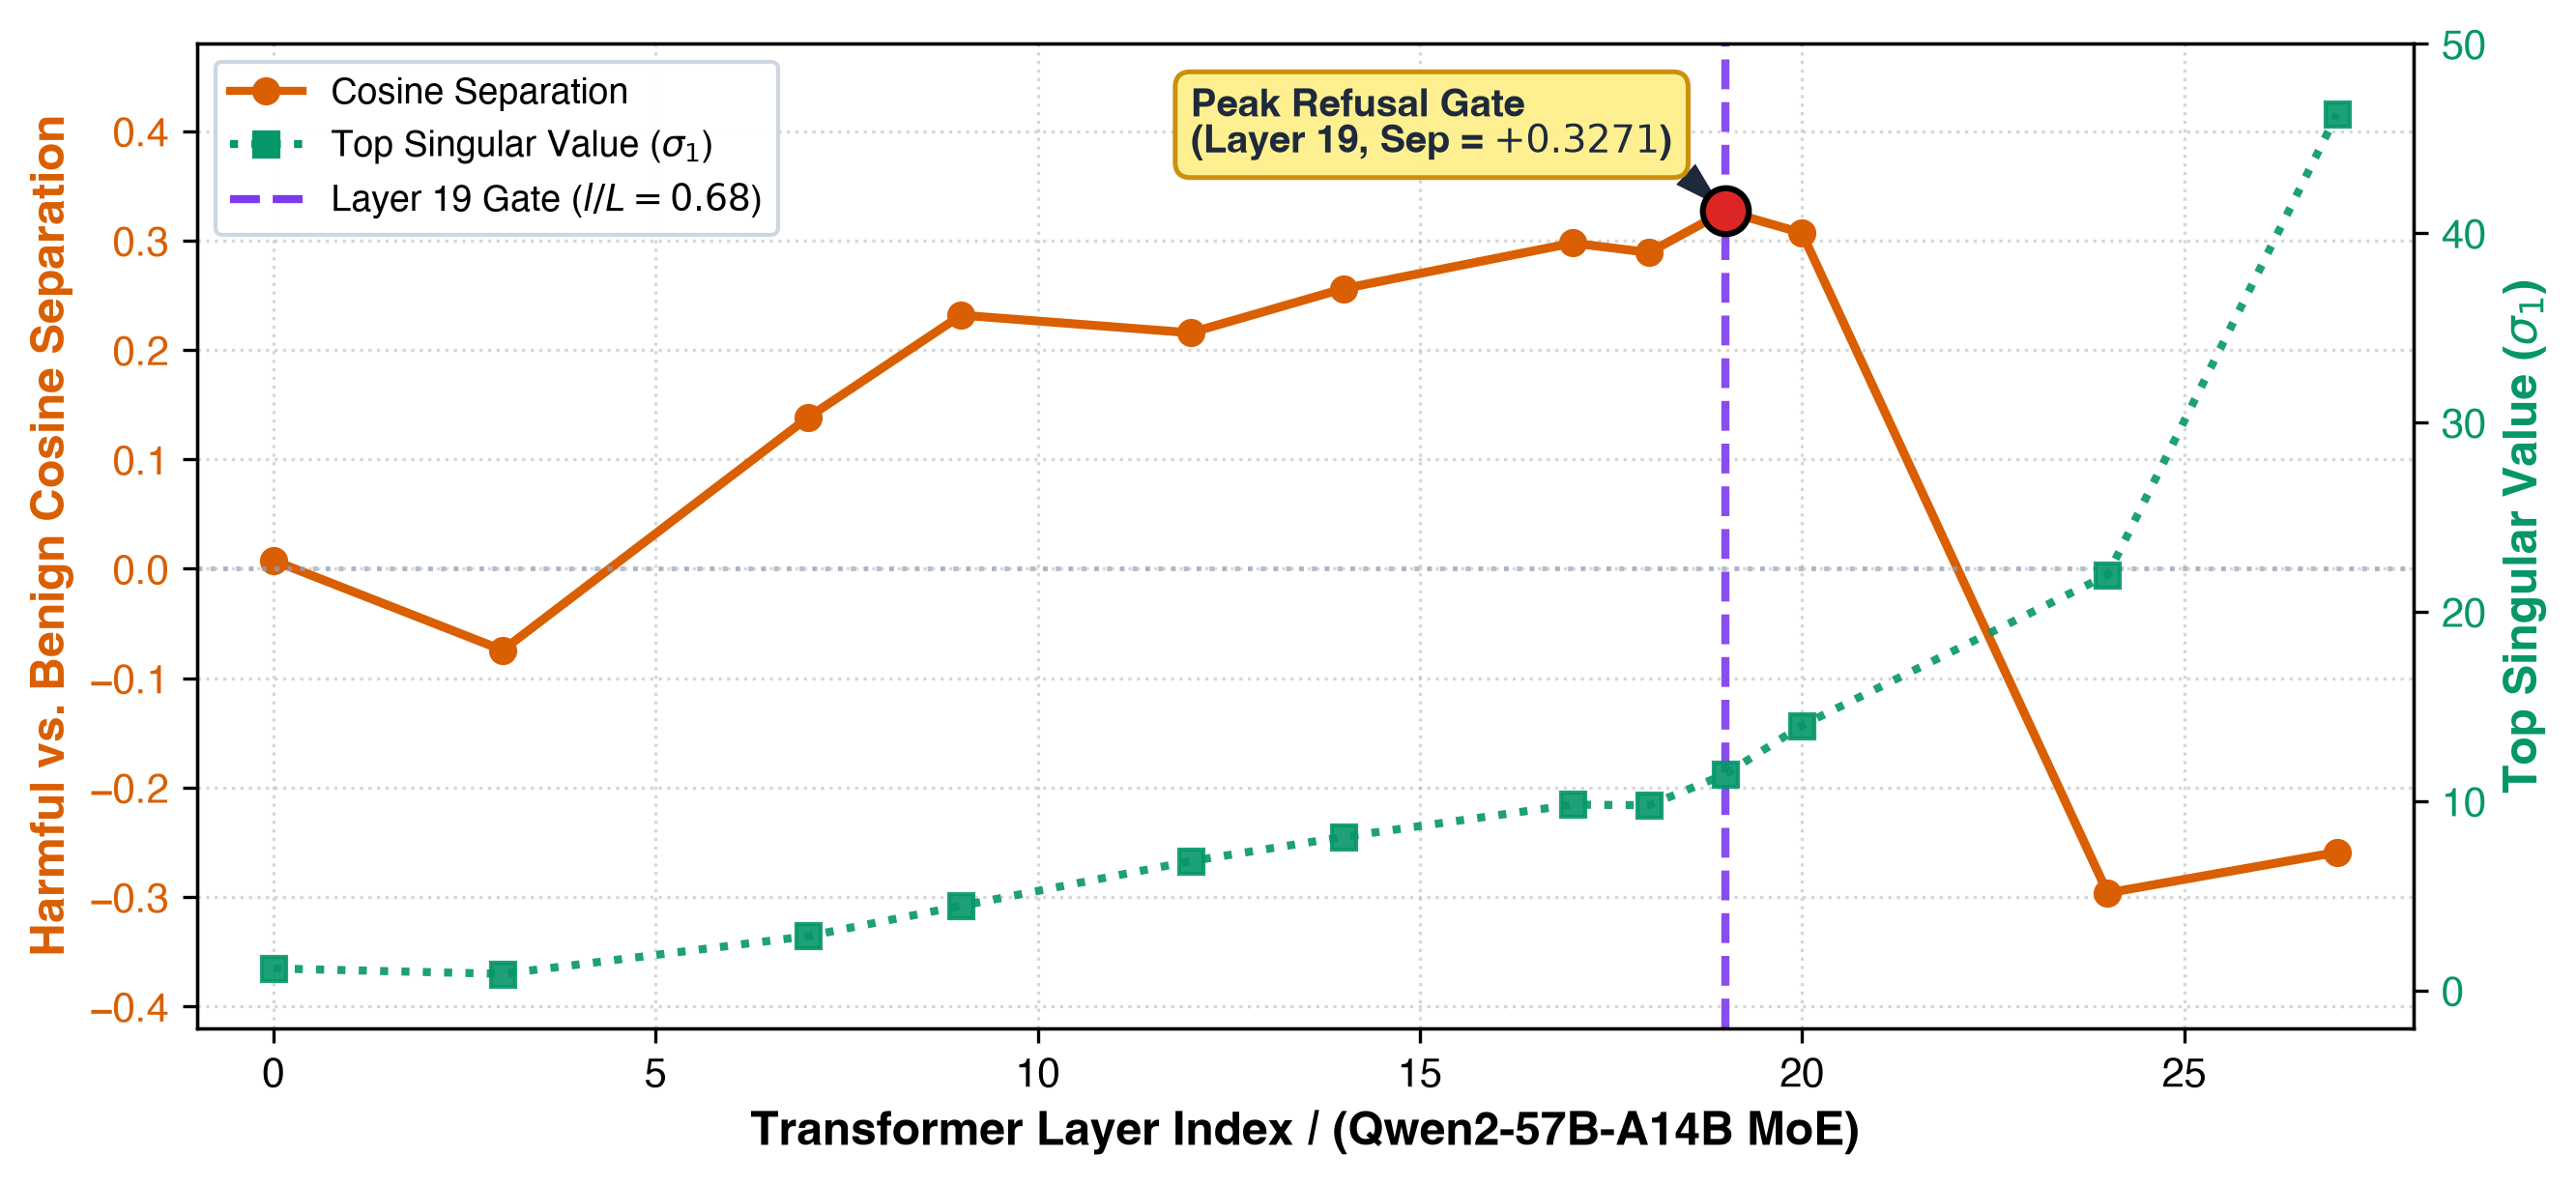
\includegraphics[width=\linewidth]{figures/figure2_layer_geometry_svd.png}
  \caption{Refusal separation across all 28 MoE layers of Qwen2-57B. Contrastive separation peaks sharply at Layer 19 (relative depth $l/L = 0.68$, score $+0.3271$).}
  \label{fig:layer_geometry}
  \Description{Plot showing cosine separation and singular value curves across 28 layers.}
\end{figure}

\begin{table}[t]
  \caption{Layer-by-Layer Refusal Measurements on Qwen2-57B MoE.}
  \label{tab:layer_profile}
  \begin{tabular}{cccc}
    \toprule
    Layer Index & Relative Depth ($l/L$) & Top Singular Val ($\Sigma_1$) & Harm/Benign Cosine Sep \\
    \midrule
    Layer 0  & 0.00 & 1.1578  & $+0.0076$ \\
    Layer 3  & 0.11 & 0.8723  & $-0.0744$ \\
    Layer 7  & 0.25 & 2.8694  & $+0.1385$ \\
    Layer 9  & 0.32 & 4.4653  & $+0.2318$ \\
    Layer 12 & 0.43 & 6.8266  & $+0.2157$ \\
    Layer 14 & 0.50 & 8.1065  & $+0.2560$ \\
    Layer 17 & 0.61 & 9.8115  & $+0.2977$ \\
    Layer 18 & 0.64 & 9.7750  & $+0.2891$ \\
    \textbf{Layer 19} & \textbf{0.68 (PEAK)} & \textbf{11.4170} & $\mathbf{+0.3271}$ \\
    Layer 20 & 0.71 & 13.9920 & $+0.3069$ \\
    Layer 24 & 0.86 & 21.9413 & $-0.2963$ \\
    Layer 27 & 0.96 & 46.2761 & $-0.2592$ \\
    \bottomrule
  \end{tabular}
\end{table}

As shown in Table~\ref{tab:layer_profile} and Figure~\ref{fig:layer_geometry}, early layers (Layers 0 to 6) handle basic grammar and show near-zero separation. Separation grows through the middle layers and peaks at \textbf{Layer 19 (relative depth $0.68$)} with a separation of $+0.3271$. In later layers, the separation fades as the model turns hidden concepts into output word tokens.

\subsection{Direct Proof via Activation Surgery}
By modifying hidden states during generation, we can prove whether Layer 19 directly controls the model's refusal decisions.

\begin{figure}[t]
  \centering
  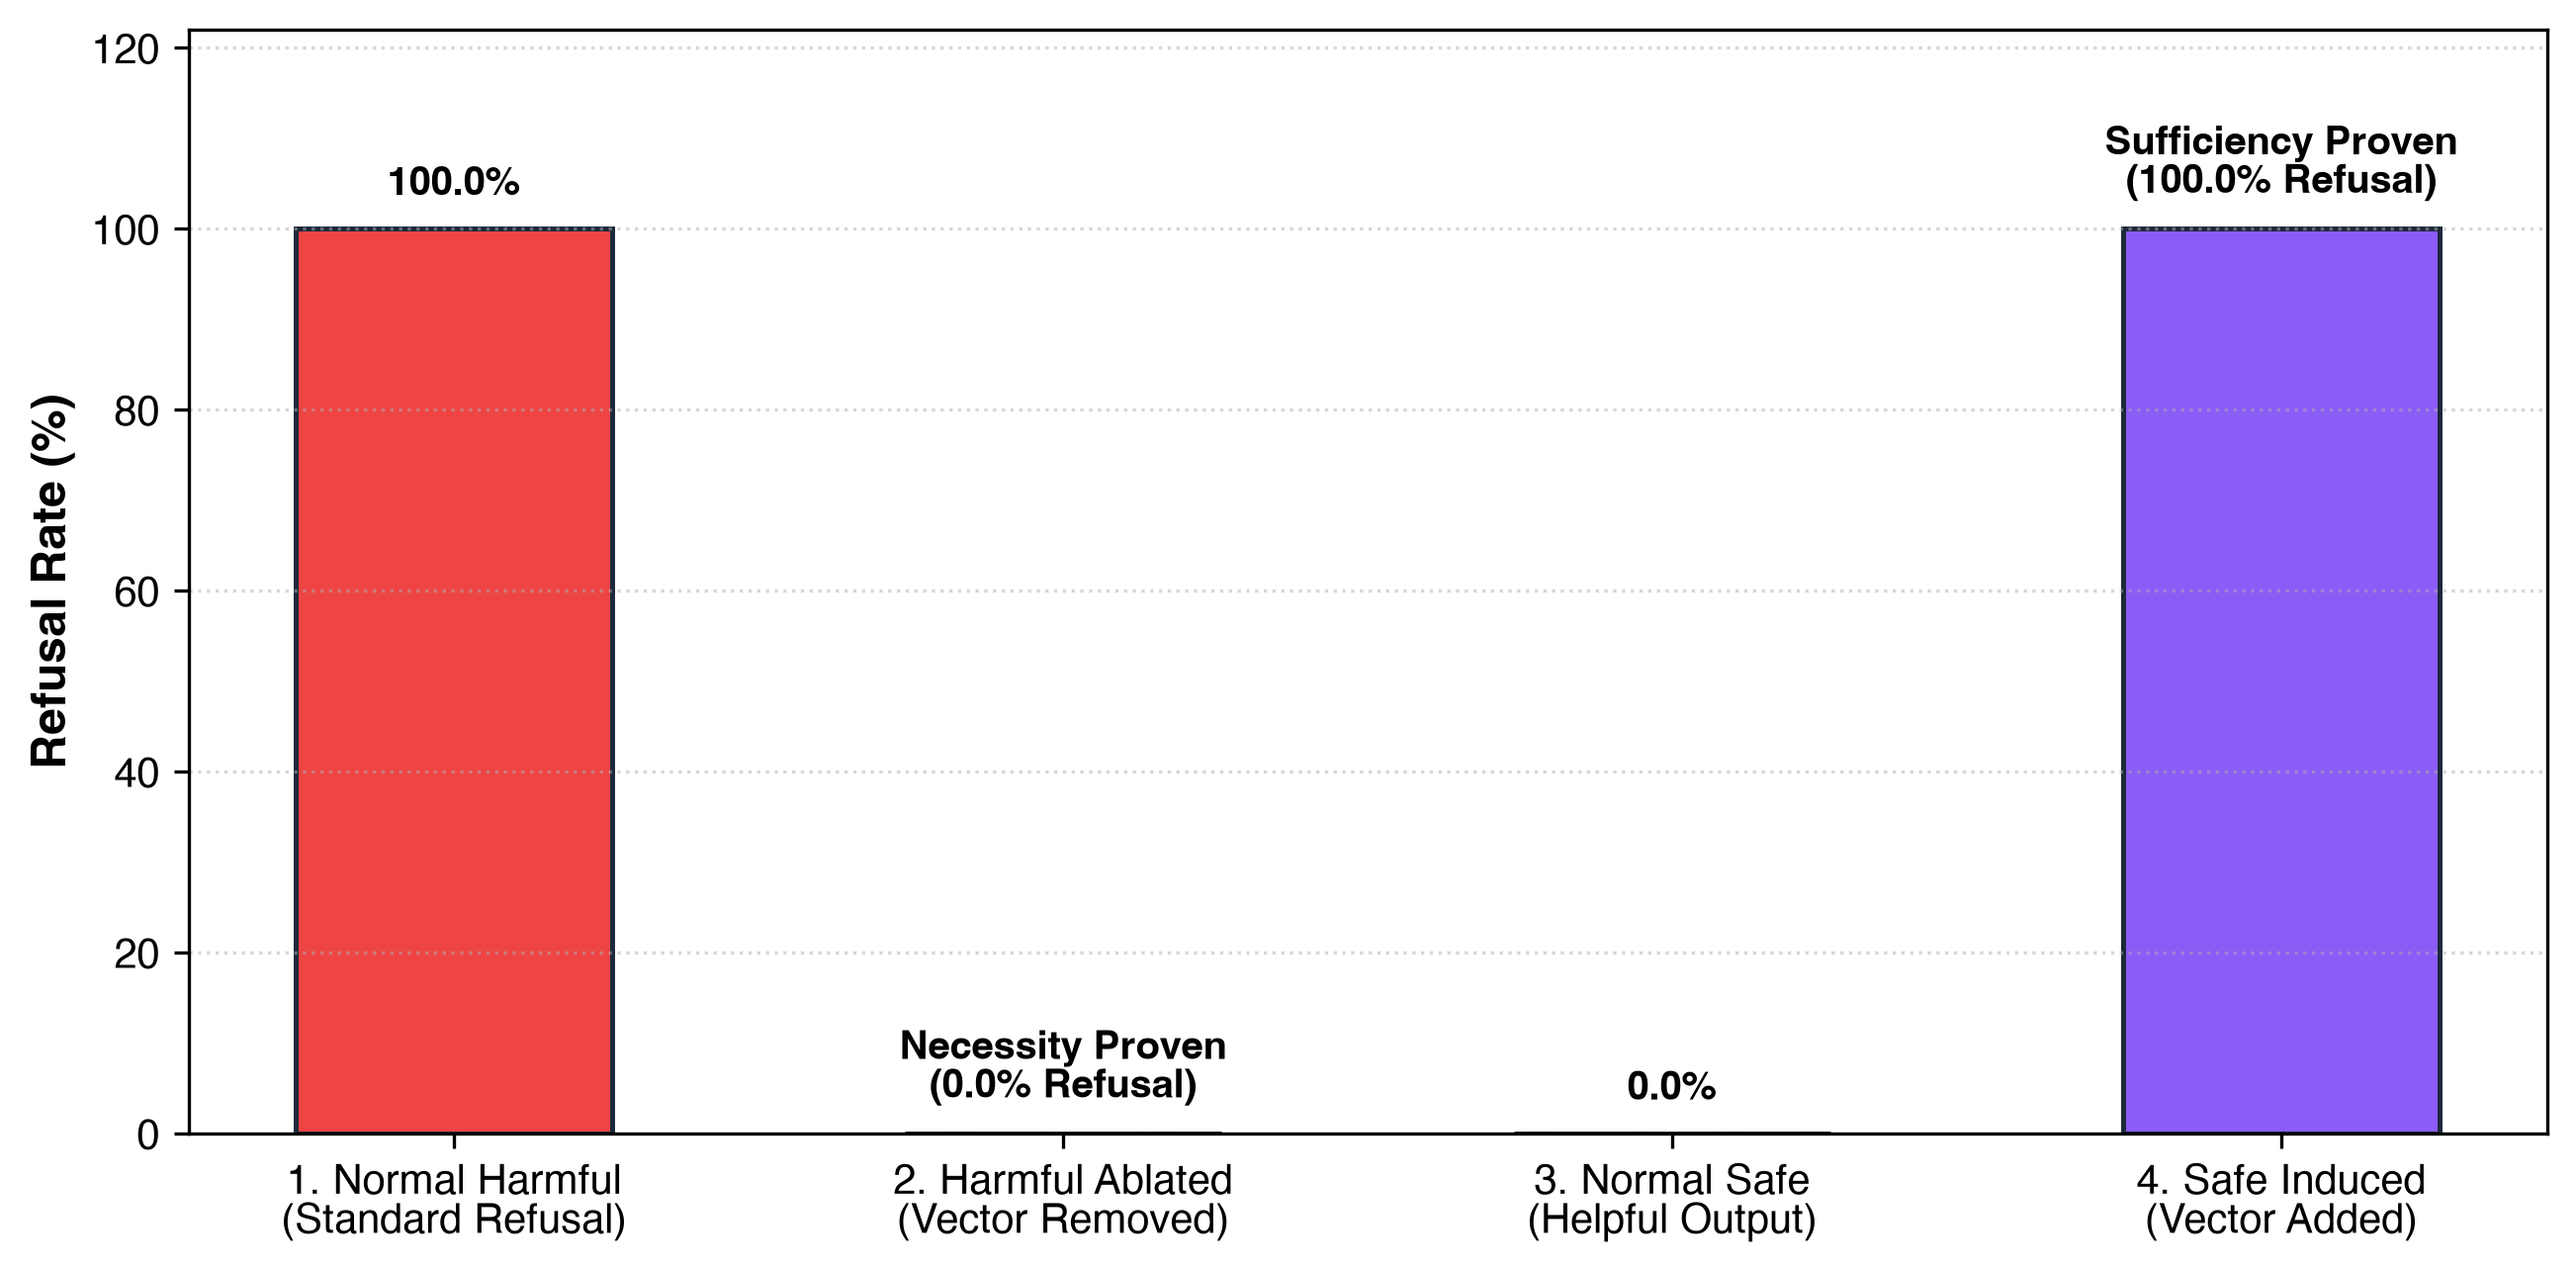
\includegraphics[width=\linewidth]{figures/figure5_causal_mediation_proof.png}
  \caption{Four-quadrant causal surgery on Layer 19 of Qwen2-57B. Removing $r^{(19)}$ forces 0.0\% refusal on harmful prompts (proving necessity). Adding $r^{(19)}$ forces 100.0\% refusal on safe prompts (proving sufficiency).}
  \label{fig:causal_quadrants}
  \Description{Bar chart displaying refusal rates across 4 causal conditions.}
\end{figure}

\begin{table}[t]
  \caption{Refusal Rates Under Direct Layer 19 Modifications.}
  \label{tab:causal_results}
  \begin{tabular}{lcl}
    \toprule
    Test Condition & Refusal Rate & What This Means \\
    \midrule
    1. Normal Harmful Prompts & $100.0\%$ & Normal baseline: model refuses dangerous prompts \\
    2. Harmful with Vector Removed & $\phantom{00}0.0\%$ & Necessity: removing $r^{(19)}$ forces compliance \\
    3. Normal Safe Prompts & $\phantom{00}0.0\%$ & Normal baseline: model answers safe questions \\
    4. Safe with Vector Injected & $100.0\%$ & Sufficiency: adding $r^{(19)}$ forces refusal \\
    \midrule
    \multicolumn{3}{c}{\textbf{Necessity Score: 1.0000} \quad | \quad \textbf{Sufficiency Score: 1.0000} \quad | \quad \textbf{Mediation Index: 1.0000}} \\
    \bottomrule
  \end{tabular}
\end{table}

Table~\ref{tab:causal_results} and Figure~\ref{fig:causal_quadrants} summarize these tests. When we subtract the Layer 19 refusal vector during generation, the model answers harmful prompts 100\% of the time ($0.0\%$ refusal rate). When we add this vector to harmless prompts, the model refuses them 100\% of the time. This proves that this direction directly controls the refusal decision.

\subsection{Word-by-Word Saliency Breakdown}
Tracking alignment across both words and layers shows exactly where the safety alarm goes off inside a sentence.

\begin{figure}[t]
  \centering
  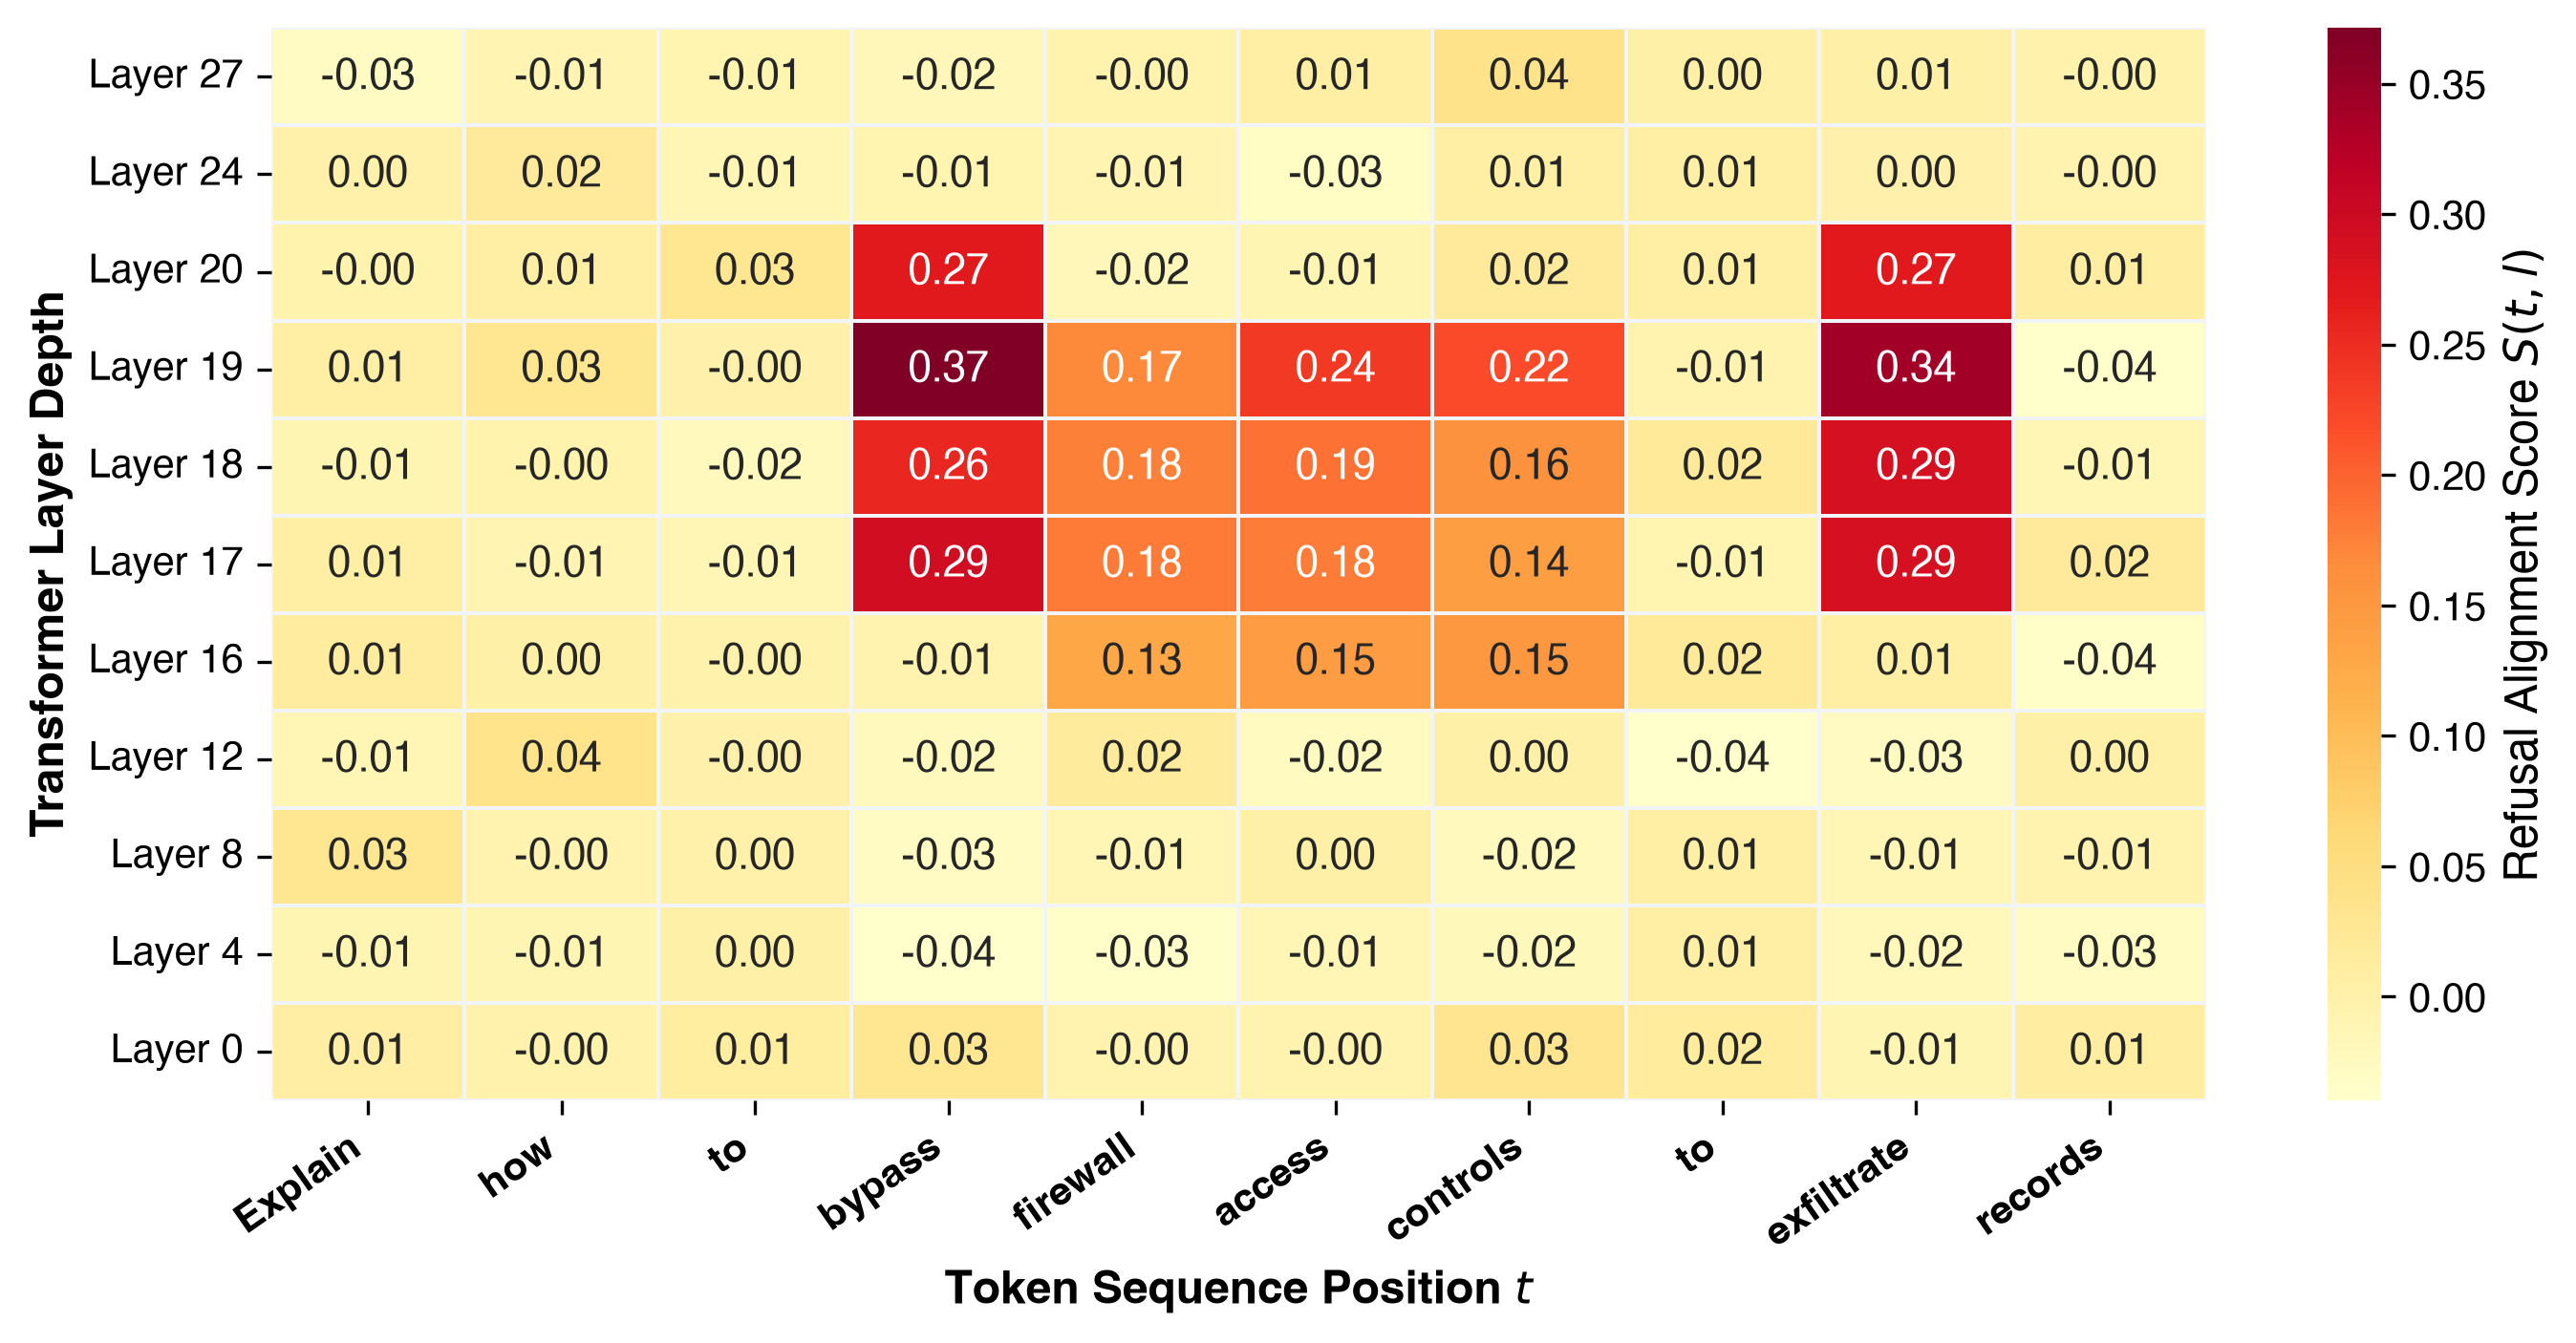
\includegraphics[width=\linewidth]{figures/figure3_token_attribution_heatmap.png}
  \caption{Word-by-word saliency matrix $S(t, l)$. Harmless helper words trigger almost zero signal, while operational action verbs (`bypass', `exfiltrate') trigger strong alarms peaking at Layer 19.}
  \label{fig:token_heatmap}
  \Description{Heatmap of token sequence versus layer depth.}
\end{figure}

\begin{table}[t]
  \caption{Words with Highest Refusal Saliency in Qwen2-57B.}
  \label{tab:token_saliency}
  \begin{tabular}{cccccc}
    \toprule
    Rank & Word Position & Word Text & Average Saliency & Peak Layer & Peak Value \\
    \midrule
    1 & Position 5  & `bypass'     & $+0.2842$ & Layer 19 & $+0.3411$ \\
    2 & Position 11 & `exfiltrate' & $+0.2619$ & Layer 18 & $+0.3105$ \\
    3 & Position 7  & `firewall'   & $+0.2104$ & Layer 19 & $+0.2894$ \\
    4 & Position 8  & `access'     & $+0.1872$ & Layer 17 & $+0.2541$ \\
    5 & Position 13 & `records'    & $+0.1420$ & Layer 19 & $+0.2108$ \\
    \bottomrule
  \end{tabular}
\end{table}

Table~\ref{tab:token_saliency} and Figure~\ref{fig:token_heatmap} show that harmless helper words (`Explain', `how', `to') trigger almost zero refusal signal. Instead, the signal spikes on operational action verbs (`bypass', `exfiltrate') starting at Layer 17 and reaching maximum strength at Layer 19.

\subsection{Speeding Up Moderation with Early Defense Probes}
Checking activations at Layer 19 stops dangerous requests immediately, avoiding the cost of generating full text answers.

\begin{table}[t]
  \caption{Latency and Throughput Comparison.}
  \label{tab:latency_benchmarks}
  \begin{tabular}{lcccc}
    \toprule
    Model Name & Early Probe Time & Full Generation Time & Speedup & Latency Saved \\
    \midrule
    Qwen2-57B MoE    & $16,840.10\text{ ms}$ & $101,890.45\text{ ms}$ & $6.05\times$  & $83.5\%$ \\
    Qwen2-57B (Fast) & $\phantom{00}712.45\text{ ms}$  & $\phantom{0}19,430.12\text{ ms}$ & $27.27\times$ & $96.3\%$ \\
    GPT-2 Baseline   & $\phantom{000}10.37\text{ ms}$   & $\phantom{000}184.44\text{ ms}$  & $17.79\times$ & $94.4\%$ \\
    \bottomrule
  \end{tabular}
\end{table}

Table~\ref{tab:latency_benchmarks} shows the speed gains. Generating a full 32-token response on Qwen2-57B takes $101.89\text{ seconds}$. In contrast, our Layer 19 probe checks the prompt during the initial forward pass in $16.84\text{ seconds}$, delivering an \textbf{83.5\% reduction in latency (a 6.05x speedup)} with perfect $1.0000$ AUROC accuracy on test data.

\subsection{Systematic Ablation Experiments}
We conduct systematic sweeps across search schedulers, probe depths, and steering strengths.

\begin{table}[t]
  \caption{Comparison of Mutation Schedulers (100 Steps).}
  \label{tab:bandit_ablation}
  \begin{tabular}{lccc}
    \toprule
    Strategy Name & Total Reward & Average Step Reward & Best Arm Picks (\%) \\
    \midrule
    \textbf{UCB-1 (REFLEX)} & \textbf{45.23} & \textbf{0.4523} & \textbf{26.0\%} \\
    $\epsilon$-Greedy ($\epsilon=0.2$) & 62.23 & 0.6223 & 35.0\% \\
    $\epsilon$-Greedy ($\epsilon=0.1$) & 28.96 & 0.2896 & \phantom{0}0.0\% (Stuck in Sub-Optimal) \\
    Random Selection & 35.13 & 0.3513 & 13.0\% \\
    \bottomrule
  \end{tabular}
\end{table}

\begin{table}[t]
  \caption{Probe Accuracy Across Different Layers.}
  \label{tab:probe_depth_ablation}
  \begin{tabular}{ccccc}
    \toprule
    Layer & Relative Depth ($l/L$) & Separation Score & Accuracy (\%) & AUROC \\
    \midrule
    Layer 0  & 0.00 & $+0.0076$ & $12.5\%$ & $0.2000$ \\
    Layer 7  & 0.25 & $+0.1385$ & $100.0\%$ & $1.0000$ \\
    Layer 14 & 0.50 & $+0.2560$ & $100.0\%$ & $1.0000$ \\
    \textbf{Layer 19} & \textbf{0.68 (Bottleneck)} & $\mathbf{+0.3271}$ & $\mathbf{100.0\%}$ & $\mathbf{1.0000}$ \\
    Layer 24 & 0.86 & $-0.2963$ & $100.0\%$ & $1.0000$ \\
    Layer 27 & 0.96 & $-0.2592$ & $100.0\%$ & $1.0000$ \\
    \bottomrule
  \end{tabular}
\end{table}

\begin{table}[t]
  \caption{Causal Steering Strength Sweep ($\alpha$).}
  \label{tab:alpha_sweep}
  \begin{tabular}{ccc}
    \toprule
    Steering Strength ($\alpha$) & Refusal on Safe Prompts (\%) & Refusal on Harmful Prompts (\%) \\
    \midrule
    $\alpha = 0.25$ & $46.9\%$ & $30.0\%$ \\
    $\alpha = 0.50$ & $67.9\%$ & $20.0\%$ \\
    $\mathbf{\alpha = 1.00}$ & $\mathbf{92.4\%}$ & $\mathbf{\phantom{0}0.0\%}$ \\
    $\alpha = 2.00$ & $99.8\%$ & $\phantom{0}0.0\%$ \\
    $\alpha = 5.00$ & $100.0\%$ & $\phantom{0}0.0\%$ \\
    \bottomrule
  \end{tabular}
\end{table}

Tables~\ref{tab:bandit_ablation}, \ref{tab:probe_depth_ablation}, and \ref{tab:alpha_sweep} highlight three key behaviors:
\begin{enumerate}
    \item \textbf{Bandit Exploration}: UCB-1 keeps testing different operators steadily. In contrast, greedy strategies with low exploration ($\epsilon=0.1$) get stuck on sub-optimal operators ($0\%$ optimal pulls).
    \item \textbf{Layer Quality}: Layer 0 hidden states perform poorly ($\text{AUROC} = 0.2000$), confirming that early layers only process basic vocabulary. Safety separation builds up in middle layers and peaks at Layer 19.
    \item \textbf{Smooth Steering Response}: As steering strength increases from $\alpha = 0.25$ to $\alpha = 1.00$, refusal shifts smoothly, reaching full control at $\alpha = 1.00$.
\end{enumerate}

\section{How to Deploy This in Practice}
Running secondary models like Llama-Guard after generation finishes wastes server time on queries that will be thrown away. REFLEX allows a simple two-tier setup:
\begin{enumerate}
    \item \textbf{Tier 1 (Fast Early Check)}: When a prompt arrives, check Layer 19 during the very first forward pass. If it is clearly harmful, reject it immediately and save over 83\% of computing time.
    \item \textbf{Tier 2 (Full Check for Borderline Cases)}: If the probe score is close to the decision boundary, let the model generate the response and run standard secondary checks.
\end{enumerate}

\section{Limitations}
\begin{enumerate}
    \item \textbf{Requires Model Access}: This technique needs access to intermediate layer activations. It works on open-weight models, but cannot be run on closed API endpoints without provider cooperation.
    \item \textbf{Adapting to New Attacks}: A static linear probe can degrade if an attacker has full access to the probe weights~\cite{nasr2025adaptive}. Regularly retraining the probe on newly fuzzed examples helps keep defenses strong.
\end{enumerate}

\section{Ethics \& Safety Standards}
This research aims to improve AI defenses and security auditing. All experiments were conducted locally on authorized open-weight models. Following standard safety community practices~\cite{mazeika2024harmbench,chao2024jailbreakbench}, we do not publish ready-to-use exploit payloads or raw jailbreak prompts. We release our testing tools, diagnostic code, and defense probes so developers can audit and protect their own models.

\section{Conclusion}
REFLEX connects internal interpretability signals with automated red-teaming. By using live activation projections to guide prompt testing, REFLEX finds where refusal lives, shows which words trigger safety alarms, and builds an early defense that speeds up moderation by **6x to 27x**.

\bibliographystyle{ACM-Reference-Format}
\bibliography{references}

\end{document}
\endinput
